\chapter[SCP-072 床脚]{
    SCP-072 The Foot of the Bed\\
    SCP-072 床脚
}

\label{chap:SCP-072}

\begin{figure}[H]
    \centering
    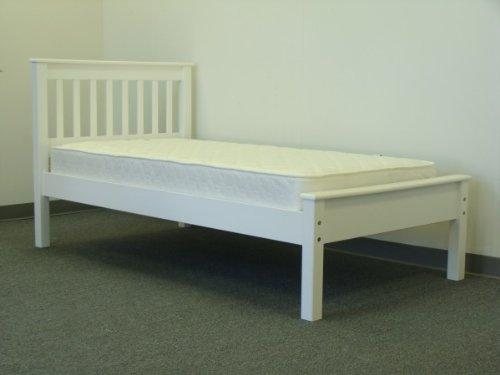
\includegraphics[width=0.5\linewidth]{images/SCP.072.jpg}
    \caption*{在从██████████公寓搬出前除去了床单被套等的SCP-072-2}
\end{figure}

\bb{项目编号:}SCP-072

\bb{项目等级:}Safe

\bb{特殊收容措施:}所有已知SCP-072实体应收容于一间3.5×4米的收容室内。仅允许在经批准的测试程序中接触对象。若无高级研究员Grant的事先许可,不得将用于使人在其上睡眠的物品带入收容室周围15米范围内。

\bb{描述:}在美国密歇根州的████████,当地媒体对SCP-072的影响的两次报道导致的恐慌引起了基金会安插的特工███████的注意。SCP-072的实体因此被首次发现。

SCP-072是一个模糊的半透明投影,像一只0.9米长的手,“手指”末端尖锐。由于其在高于5勒克斯的照度下不可见,难以记录SCP-072的清晰影像。

观察显示SCP-072实体仅在一名人类(下文以“实验对象”代指)在一张被SCP-072“感染”的床上进入快速眼动睡眠并将脚伸到被子外面时显现。若满足以上条件,SCP-072将从床脚中伸出并似乎用其食指“轻触”实验对象的脚直到对象醒来。实验对象报告他们在此时无法移动,这与睡眠麻痹(译注:或译作睡眠瘫痪症,即“鬼压床”)的症状相似。只要SCP-072可见,该状况就将持续。

SCP-072之后将用其尖锐的手指从实验对象脚暴露在外的部分切下成份的肉。每次切除之间它返回床内,出来时其收集到的材料消失了。该过程持续到SCP-072带走整只或两只露出的脚,到踝部为止。虽然接触SCP-072的实验对象称该过程极其疼痛,但其麻痹效果使他们无法尖叫或呼救。不清楚显现的SCP-072是以得到的材料为食还是将其用于其它目的。只要伤口处理得当,SCP-072的效果将不会致命,但已观察到这在之后导致了睡眠方面的心理创伤。

同时存在一个次要影响:在一张展现出SCP-072效果的床附近约10米内的任何床同样会被一个SCP-072实体寄宿。摧毁被SCP-072影响的床后找不到异常材料,也没有从实验对象身上取下的生物原料的踪迹。

\bb{附录}\\
已知SCP-072项目列表:\\
\bb{SCP-072-1}、\bb{-2}和\bb{-3},从最初(发生事件)的公寓建筑群中回收,为三张双人床,之前的相互距离都在10米内。\\
\bb{SCP-072-4},一张特大号的四帷柱床,在SCP-072归类为Site-██的临时异常对象藏品期间被影响。\\
\bb{SCP-072-5},一个去掉了底部的睡袋,为了测试而受到SCP-072-1影响。当D-2191在其中进入快速眼动睡眠时,{[}数据删除]。不建议在将来的测试中使用SCP-072-5。\\
\bb{SCP-072-6}和\bb{-7},受SCP-072-2影响的床,之后为进行检查而被销毁。SCP-072-6和-7的残骸似乎未被影响,但在完成进一步研究之前应继续收容。
